\section{実験のセットアップ}
\subsection{セットアップ・及び実験原理}
$\mu$を検出しアナログ信号に変えるために用いた装置は以下のものからなっている。
\begin{itemize}
\item プラスチックシンチレータ($100\,\mathrm{cm} \times 48\,\mathrm{cm} \times1\,\mathrm{cm}$)\,2枚
\item プラスチックシンチレータ($50\,\mathrm{cm} \times 5\,\mathrm{cm} \times 1\,\mathrm{cm}$)\,7枚
\item 光電子増倍管(PMT)\,2本
\item コイル(詳細は後述)\,1つ
\item 銅板($50\,\mathrm{cm} \times 48\,\mathrm{cm} \times 1\,\mathrm{cm}$)\,1つ
\item MPPC及びそのための基盤(詳細は後述)\,7つ
\item 光ファイバー\,7本
\end{itemize}
以上の装置を$\mu$の寿命測定(以下実験a)については図1、$\mu$の$g$因子測定(以下実験b)については図2にそれぞれ配置した。
\begin{figure}[H]
\centering
  \includegraphics[width=10cm, bb=0 0 996 664,clip]{jikken1.jpg}
  \caption{実験a}
\end{figure}

\begin{figure}[H]
\centering
  \includegraphics[width=10cm, bb=0 0 1031 687,clip]{jikken2.jpg}
  \caption{実験b}
\end{figure}

ここで、A,B,Cはいずれもプラスチックシンチレータである。
上記の装置で$\mu$は、以下のような振る舞いを行う。
\begin{enumerate}
\item $\mu$がどこからか降って来て、AとBを突き抜け、銅板にたどり着く。
\item 銅板にたどり着いた$\mu$はエネルギーが高い場合突き抜け、Cまでたどり着くが、あるエネルギー程度の$\mu$はCu板で止まる。
\item 2で銅板で止まった$\mu$は時間が経過すると弱い相互作用によって崩壊する。
\item 3で生じた陽電子がB、またはCにたどり着く。
\end{enumerate}
なお、実験aとbのそれぞれのセットアップでMPPCとPMT0の距離を変えたのは、aでは$\mu$のカウント数をなるべく増やして統計誤差を減らすために狭く設定したが、bではシンチレータに対してスピンの方向が垂直な向きであることを仮定しているので、あまり上のシンチレータと銅板との間隔が狭いと斜めからの$\mu$が入り込んでしまうことも考慮して、aより広く間隔を設定した。
\subsection{実験の回路図}
回路図を図3に示す。
\begin{figure}[H]
  \centering
  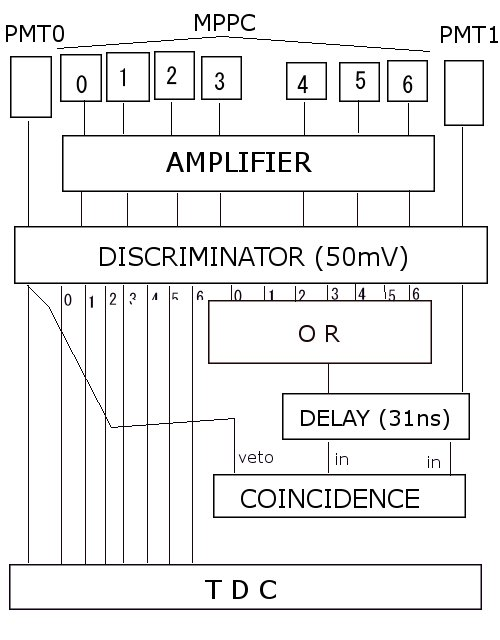
\includegraphics[width=100mm, bb=0 0 500 640]{kairo2.jpg}
  \caption{実験回路図}
\end{figure}
なお、この回路図でdelay31nsを組んでいるのは、MPPCとPMT0、PMT1の信号をCOINCIDENCEでタイミングを合わせるためである。
この回路を論理記号を用いて表すと、
\begin{itemize}
  \item Start信号:\ PMT0 $\land$ MPPC $\land$ ($\lnot$ PMT1)
  \item Stop信号0$\sim$6:\  MPPC 0$\sim$6
  \item Stop信号7:\ PMT1
\end{itemize}
となる。

\subsection{コイル}
  本実験の$g$因子測定において、磁場をコイルから発生させた。コイルは2004年度P1の課題研究用に作成されたものを使用した。このコイルはMainコイルとして4つのコイルを並列でつないだものを並べ、さらに2つのSubコイルを用いたものを使用した。
Mainコイルには31.0Vで19.0A、sub1コイルには3.5Vで0.80A、sub2コイルには3.6Vで0.80Aの電流を流した。
磁場の測定では、コイルに電流を流してから十分時間が経過して磁場が安定したあと、銅板が入っている部分を図4のように16のセクションに分け、それぞれの場所においての磁場を計4回測定した。
\begin{figure}[H]
 \begin{center}
  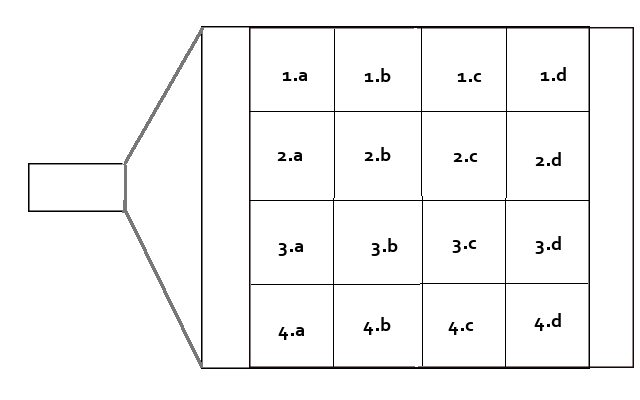
\includegraphics[width=10cm,bb=0 0 640 500]{coil.jpg}
  \caption{コイルの区分け}
 \end{center}
\end{figure}

その測定結果を表1に記す。
\begin{table}[H]
\begin{center}
\begin{tabular}{c|cccc}\hline
  セクション&1回目[Gauss]&2回目[Gauss]&3回目[Gauss]&4回目[Gauss]\\ \hline
  1.a & 51.0 & 47.0 & 49.4 & 53.8  \\
  1.b & 53.0 & 50.1 & 53.6 & 54.7  \\
  1.c & 51.6 & 50.4 & 50.2 & 50.8  \\
  1.d & 49.6 & 49.7 & 49.6 & 50.0  \\
  2.a & 54.7 & 49.2 & 52.0 & 45.5  \\
  2.b & 55.2 & 49.5 & 50.2 & 53.3  \\
  2.c & 53.2 & 49.0 & 48.7 & 49.1  \\
  2.d & 50.2 & 49.8 & 49.9 & 53.4  \\
  3.a & 51.2 & 48.8 & 49.4 & 41.7  \\
  3.b & 50.2 & 48.9 & 49.2 & 48.0  \\
  3.c & 49.8 & 48.3 & 50.5 & 47.2  \\
  3.d & 49.6 & 47.7 & 48.9 & 46.7  \\
  4.a & 50.6 & 48.0 & 49.3 & 46.2  \\
  4.b & 49.2 & 49.4 & 49.8 & 47.4  \\
  4.c & 51.5 & 47.4 & 48.0 & 45.6  \\
  4.d & 49.8 & 48.4 & 49.3 & 46.9  \\
  ave.& 51.3 & 48.9 & 49.5 & 48.8  \\
\end{tabular}
\end{center}
\end{table}
この測定結果から磁場を計算すると、$B$=49.7$\pm$3.5Gaussを得た。


\subsection{TDCの較正}
本実験では、寿命をTDCモジュールを用いて測定したので、TDCの1countが何nsか、clock generatorとオシロスコープを用いて調べた。その結果を下の表にまとめる。
\begin{table}[H]
  \begin{center}
    \begin{tabular}{c|c} \hline
      channel & ns/count \\ \hline
      ch0 &  $7.68\times 10^{-4}\pm 6.30\times 10^{-7}$ \\
      ch1 &  $7.68\times 10^{-4}\pm 7.41\times 10^{-7}$ \\
      ch2 &  $7.69\times 10^{-4}\pm 5.41\times 10^{-7}$ \\
      ch3 &  $7.68\times 10^{-4}\pm 6.50\times 10^{-7}$ \\
      ch4 &  $7.64\times 10^{-4}\pm 1.62\times 10^{-6}$ \\
      ch5 &  $7.63\times 10^{-4}\pm 8.63\times 10^{-7}$ \\
      ch6 &  $7.63\times 10^{-4}\pm 1.04\times 10^{-6}$ \\
      ch7 &  $7.63\times 10^{-4}\pm 8.64\times 10^{-7}$ \\
    \end{tabular}
  \end{center}
\end{table}
\subsection{PMT(光電子増倍管)・及びDiscriminatorの設定}
ここで、$\mu$の寿命測定及び$g$因子測定で用いたPMTの電圧・及びDiscriminatorの設定の過程を述べる。
\subsubsection{Discriminatorの閾値設定}
まず、本実験で用いたDiscriminatorの閾値の設定方法について述べる。この閾値をうまく設けることでPMT及びMPPCからの信号のうちバックグラウンドのイベントをシャットアウトし、検出したい$\mu$の信号のみを検出することができる。
本実験では、まず最初にMPPCとPMT両方のDiscriminatorの閾値を30mVに設定し、他のノイズをシャットアウトできるように、またgainが揃うようにそれぞれ1700V、1750Vとして測定を開始した。しかし、この測定結果のグラフを見たところ、これはDiscriminatorの閾値が低く、$\mu$以外のバックグラウンドも検出していると判断し、Discriminatorの閾値を決めなおした。その際、今度はMPPCの$\mu$の信号をそれぞれオシロスコープで見たところほぼ60mVでそろっていたので、Discriminatorの閾値を59mVで設定しなおした。
また、Stop信号がMPPC、PMT1それぞれに来ている割合を見ると、PMT1にほとんど信号が来ていなかったので、これはPMTの電圧設定が低すぎて$\mu$の信号が検出できてないことが原因と判断し、PMTの電圧設定をPMT0、PMT1それぞれ1949V、1998Vと高く設定しなおし、バックグラウンドをシャットアウトするために、Discriminatorの閾値を59mVに上げた。
